\section{Mainchain}\label{sec:mainchain}

Here we describe the details of the mainchain state machine (SM) controlling a
Hydra head (see Fig.~\ref{fig:SM_states_basic}) using the CEM abstraction \&
notation (see Section~\ref{sec:cem}). In addition of standard CEM modelling, we
also provide the formal conditions $\cemTxCon$ which a transition need to
satisfy and also include them in the accompanying text.

% TODO: no generic OCV anymore
% \dparagraph{Onchain verification algorithms.} The status of the head
% is maintained in a variable $\eta$, which is part of the SM state and
% updated by so-called \emph{onchain verification (OCV) algorithms}
% $\ocvInitial$, $\ocvClose$, $\ocvContest$, and $\ocvFinal$. In the context
% of the mainchain protocol, these OCV algorithms are intentionally kept
% as generic as possible; this keeps the mainchain SM compatible with
% many potential head-protocol variants.
% The concrete OCV algorithms for the head protocol specified in this
% paper are given in context of the head protocol itself as they depend
% on the specific head-protocol internals: verification of head-protocol
% certificates and related onchain state updates.
% As such, the OCV algorithms can be seen as abstract mainchain algorithms
% implemented by the specific head protocol. Consequently, the OCV
% implementation for our head protocol is described in Section~\ref{sec:hpocv}.

\begin{figure}[h]

  \centering

  % 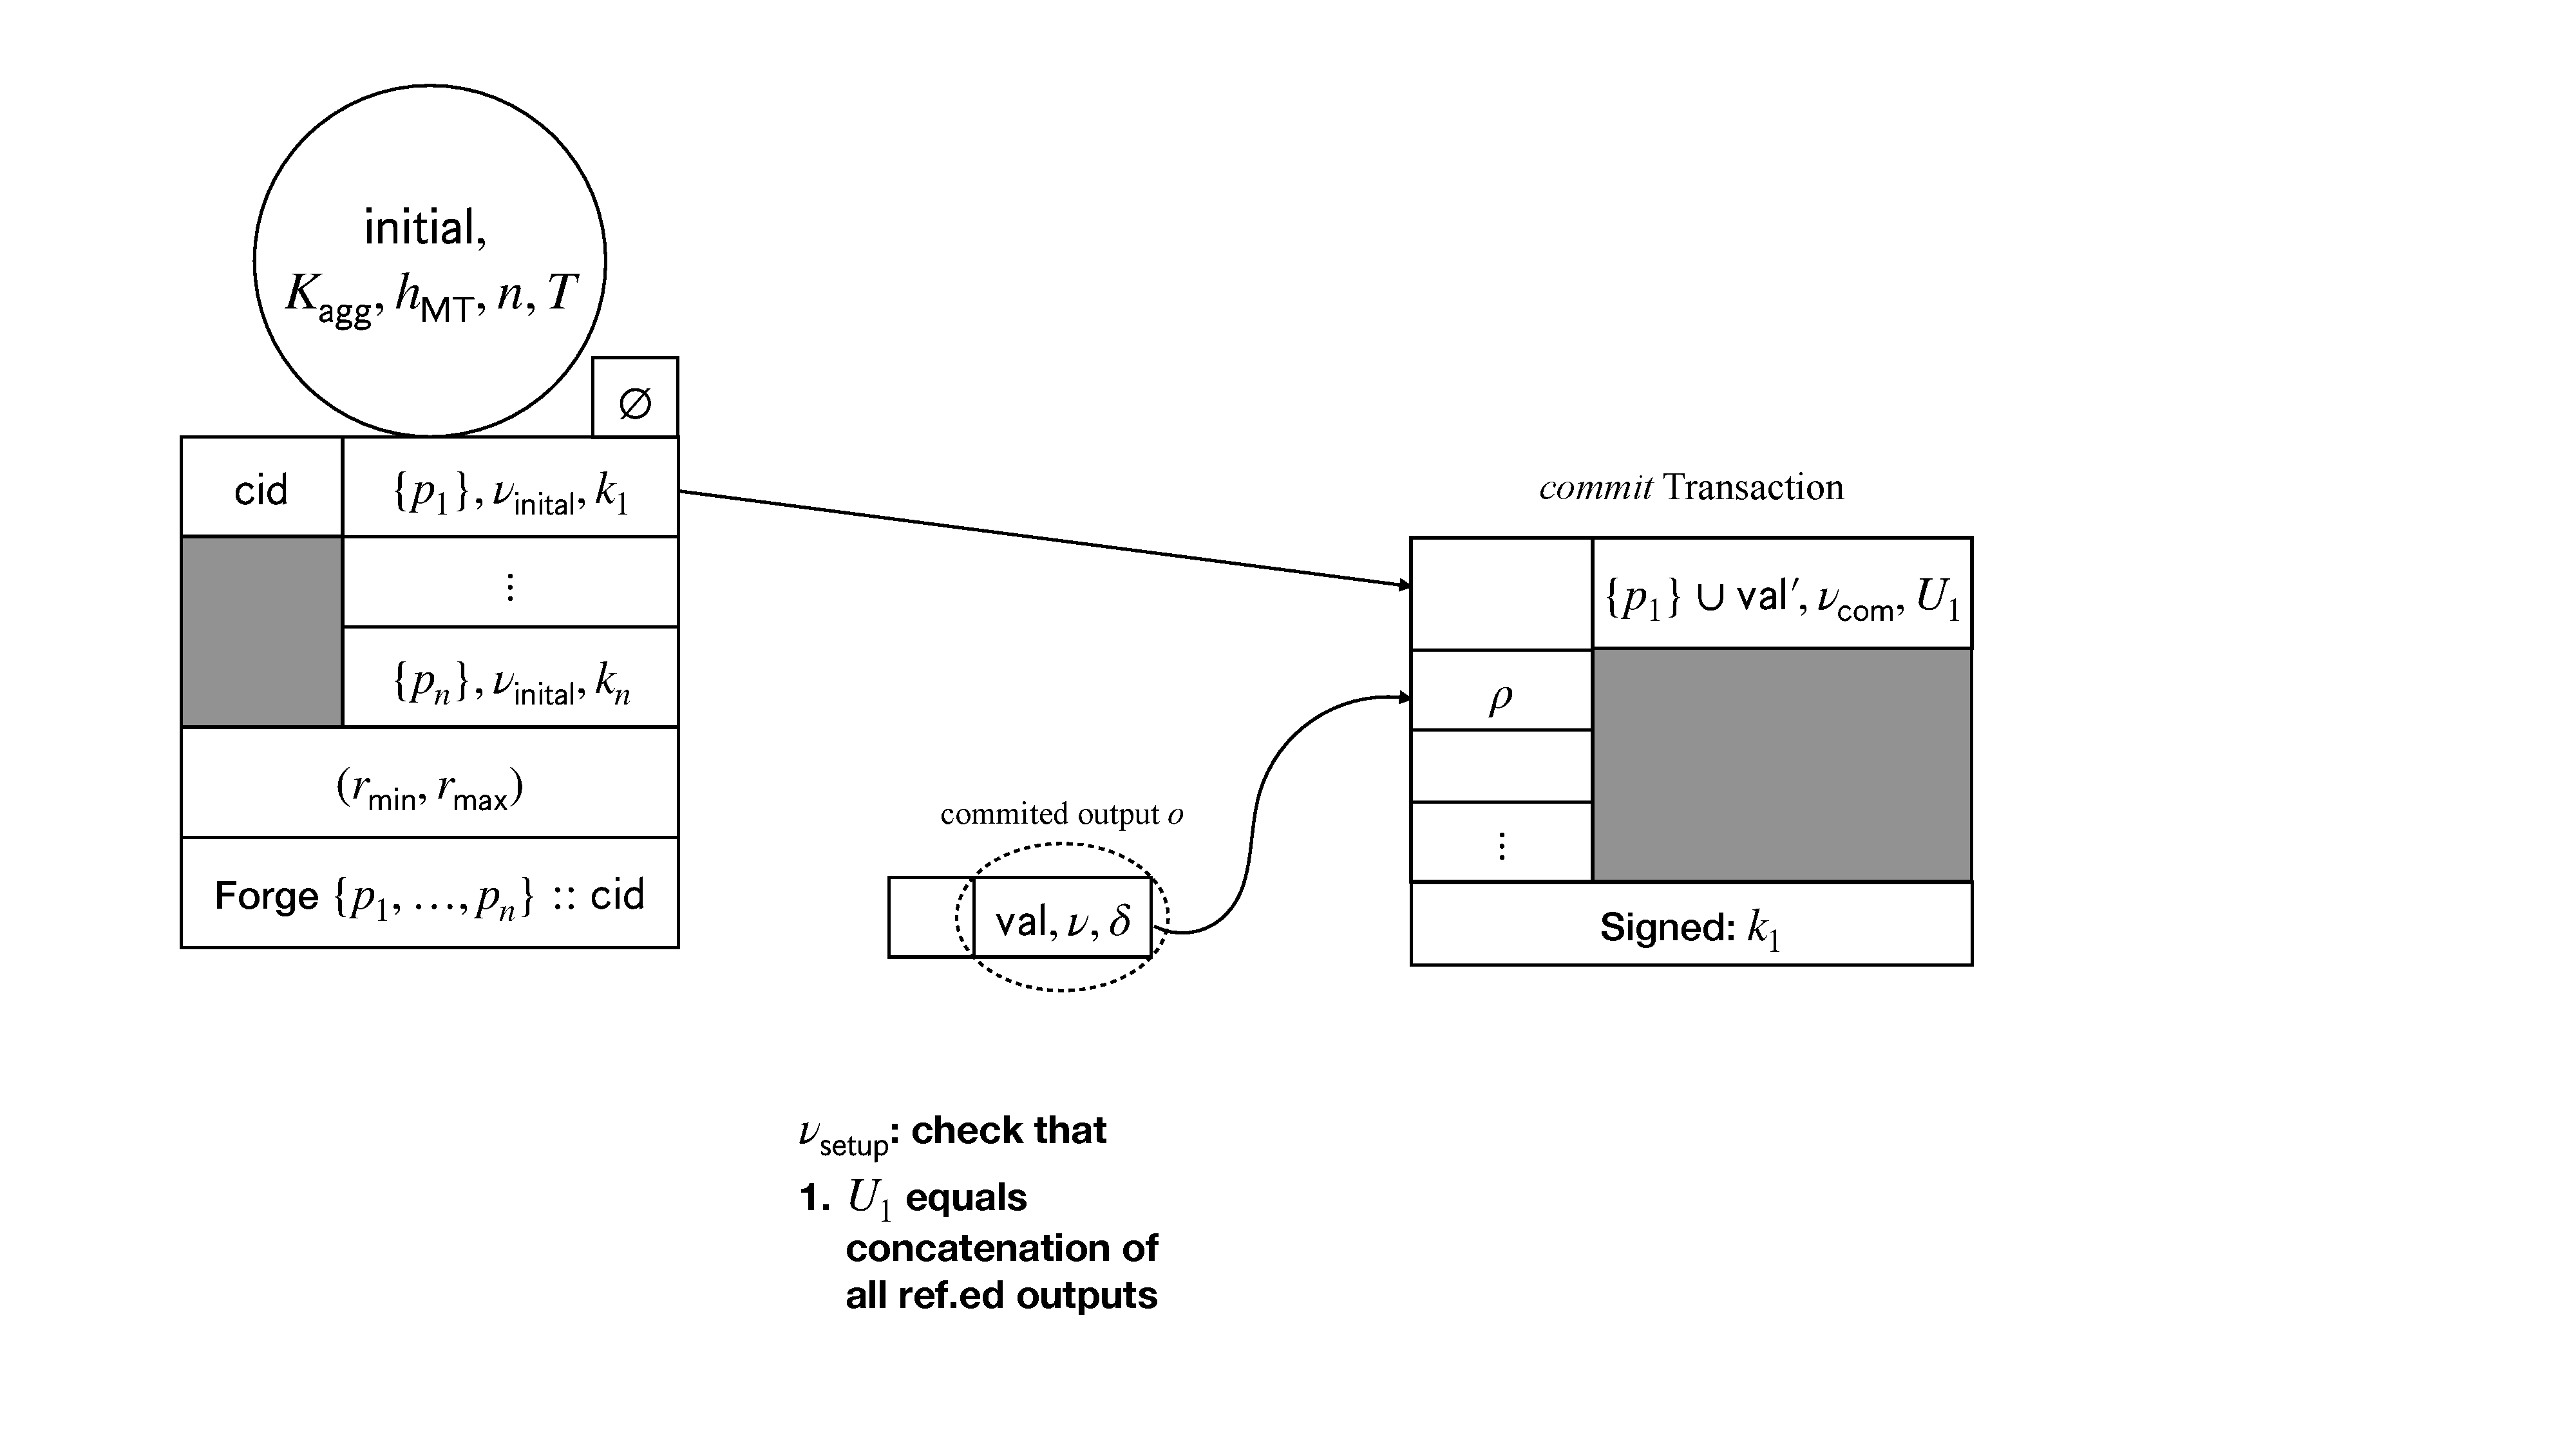
\includegraphics[width=\textwidth/2,trim=130 330 430 50,clip]{figures/SM_commit_tx.pdf}

  % TODO: clean draw marked up version
  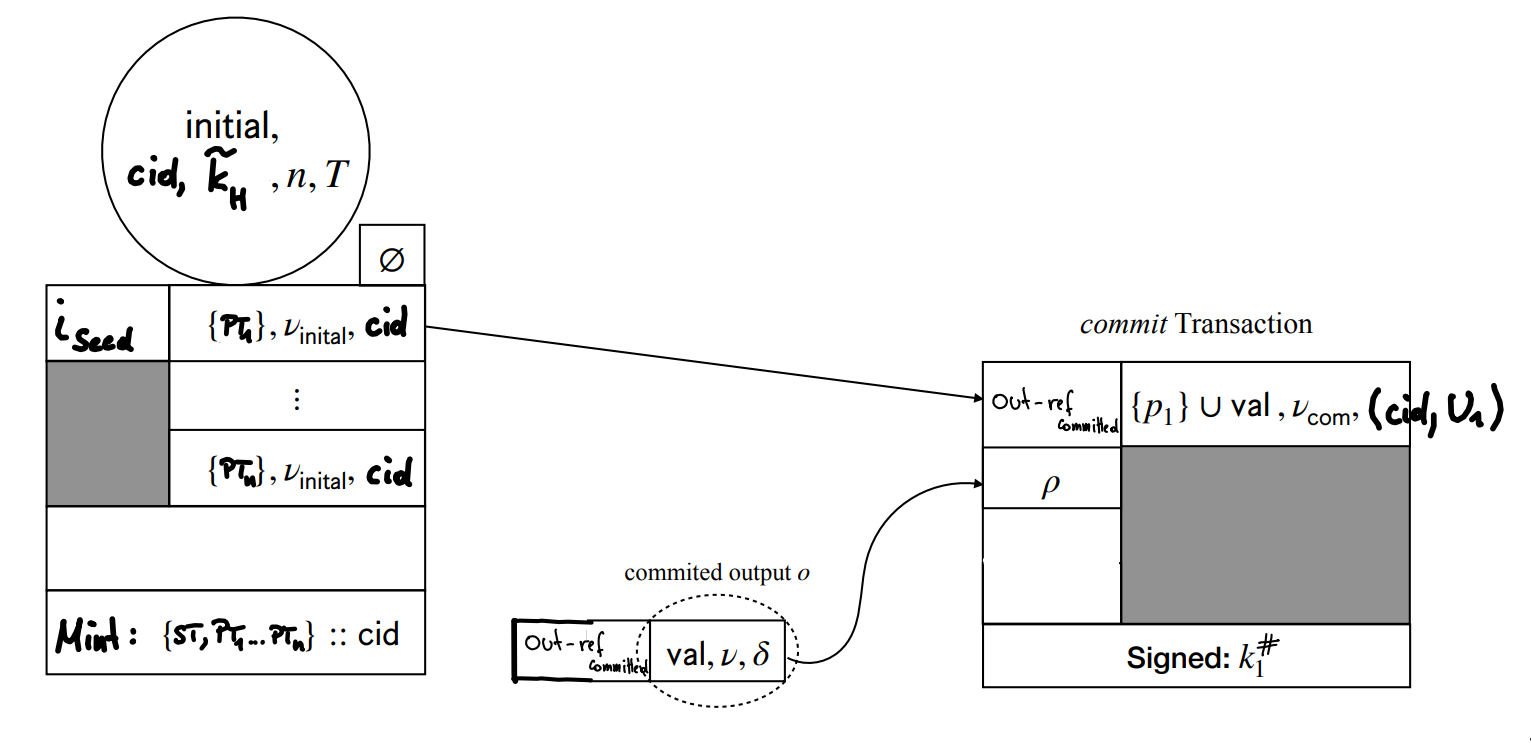
\includegraphics[width=\textwidth*2/3]{figures/SM_commit_tx.png}

  \caption{
    \mtxInit{} transaction (left) with one \mtxCom{} transaction
    (right) attached locking one output (center).}\label{fig:SM_commit_tx}

\end{figure}


%%% Local Variables:
%%% mode: latex
%%% TeX-master: "main"
%%% End:


\dparagraph{Initial state.} After the setup phase of Section~\ref{sec:hpsetup},
the head initiator posts an \mtxInit{} transaction (see
Fig.~\ref{fig:SM_commit_tx}). The \mtxInit{} transaction establishes the SM's
initial state \( (\stInitial,\hpAK,\hppuv,\nop,\cPer), \) where $\stInitial$ is
a state identifier, $\hpAK$ is the aggregated multisignature key established
during the setup phase, $\hppuv$ is the list of all participants verification
keys $(k_1,\ldots,k_\nop)$ exchanged during the setup phase and identifying the
head members, $\nop$ is the number of head members, and $\cPer$ is the length of
the contestation period. The \mtxInit{} transaction also mints $\nop$
participation tokens $\{p_1,\ldots,p_\nop\} :: \mathsf{cid}$, where the currency
ID $\mathsf{cid}$ is defined by the unique \emph{monetary-policy script}
$\muHead$.

The script is unique as it is parameterized by a \emph{seed} input, which is
checked to be spent in the script \todo{add formal notation} and the ledger
prevents double spending. Consequently, we can use $\mathsf{cid}$ as a unique
identifier for the newly initialized head. Two kinds of tokens are minted using
$\muHead$:
\begin{itemize}
\item ST: A single state thread token to ensure contract continuity \todo{ref}, the token name is a well known string, e.g. “HydraHeadV1”
\item PT: One participation token per participant, where the token name is the participant's verifikation key hash $H(k_i)$. This will be used to authenticate participants in protocol transactions.
\end{itemize}


Crucially, the \mtxInit{} transaction has $\nop$ outputs, where each output is
locked by a validator $\nuInitial$ and the $\ith i$ output has the participation
token $p_i$ in its value, while the datum is unused. Validator $\nuInitial$
then ensures that the output is consumed by

\begin{menumerate}
  \item an \mtxAbort{} transaction (see below) or
  \item a \mtxCom{} transaction (identified by having validator $\nuCom$ in its
  only output\todo{highlight this?}), and
  \begin{menumerate}
    \item the transaction is signed and the signature verifies as valid with
    verification key corresponding to the asset name in $p_i$,
    \item the redeemer for $\nuInitial$ is referencing the output to commit $ \rho = \txOutRef_{commit}$, with output $o_{commit}$ holding value $\val_{commit}$
    \item the committed value is in the output $\val' = \{p_{i}\} \cup \val_{commit} $,
    \item the data field $\delta$ of the single commit transaction output includes\todo{also cid} \\
    $U_i = \recordUTxO(\txOutRef_{commit},o_{commit})$, where and $\recordUTxO$
    stores output references and outputs in a canonical way, \todo{define
      recordUTxO}
    \item the data field includes $\mathsf{cid}$, \todo{from GDoc}
    \item no minting or burning happens.
  \end{menumerate}
\end{menumerate}

The general well-formedness and validity of the \mtxInit{} transaction is
checked on the mainchain, including the fact that the committed output
$o_{commit}$ can be spent. The head members additionally check whether the head
parameters match the parameters agreed on during the setup phase. In case of a
mismatch the head opening is considered as failed.

\dparagraph{Committing outputs to a head.} To lock outputs for a Hydra head, the
$\ith i$ head member will attach a \mtxCom{} transaction (see
Fig.~\ref{fig:SM_commit_tx}) to the $\ith i$ output of the \mtxInit{}
transaction, by picking a UTxO to commit via the redeemer $\rho$ which pinpoints
to the output to commit\footnote{Note that in this specified version of the Head
  protocol, only one output can be committed by a head participant. This is to
  avoid too big / expensive \mtxCollect{} transactions.}. The \mtxCom{}
transaction has a single output which is locked by the $\nuCom$ validator.

While the $\nuInitial$ validator ensured that the \mtxCommit{} transaction
correctly records the committed UTxO set $U_i$, the $\nuCom$ validator only
checks that the output is collected by a Hydra head transaction -- either
\mtxCCom{} or \mtxAbort{} -- using the state thread (ST) token:

\begin{menumerate}
  \item for spending via \mtxCom{} transaction
    \begin{menumerate}
      \item the ST token is present in the output value $\{cid \rightarrow ST \rightarrow 1\} \subseteq \val'$
      \item with the correct $\mathsf{cid}$ in the datum $(cid,.) = \delta$.
    \end{menumerate}
  \item for spending via \mtxAbort{} transaction
    \begin{menumerate}
      \item the ST token is getting burned $\{cid \rightarrow ST \rightarrow -1\} \subseteq \mathsf{Mint}$
      \item with the correct $\mathsf{cid}$ in the datum $(cid,.) = \delta$.
    \end{menumerate}
\end{menumerate}

\begin{figure}[h]

  \centering

  % 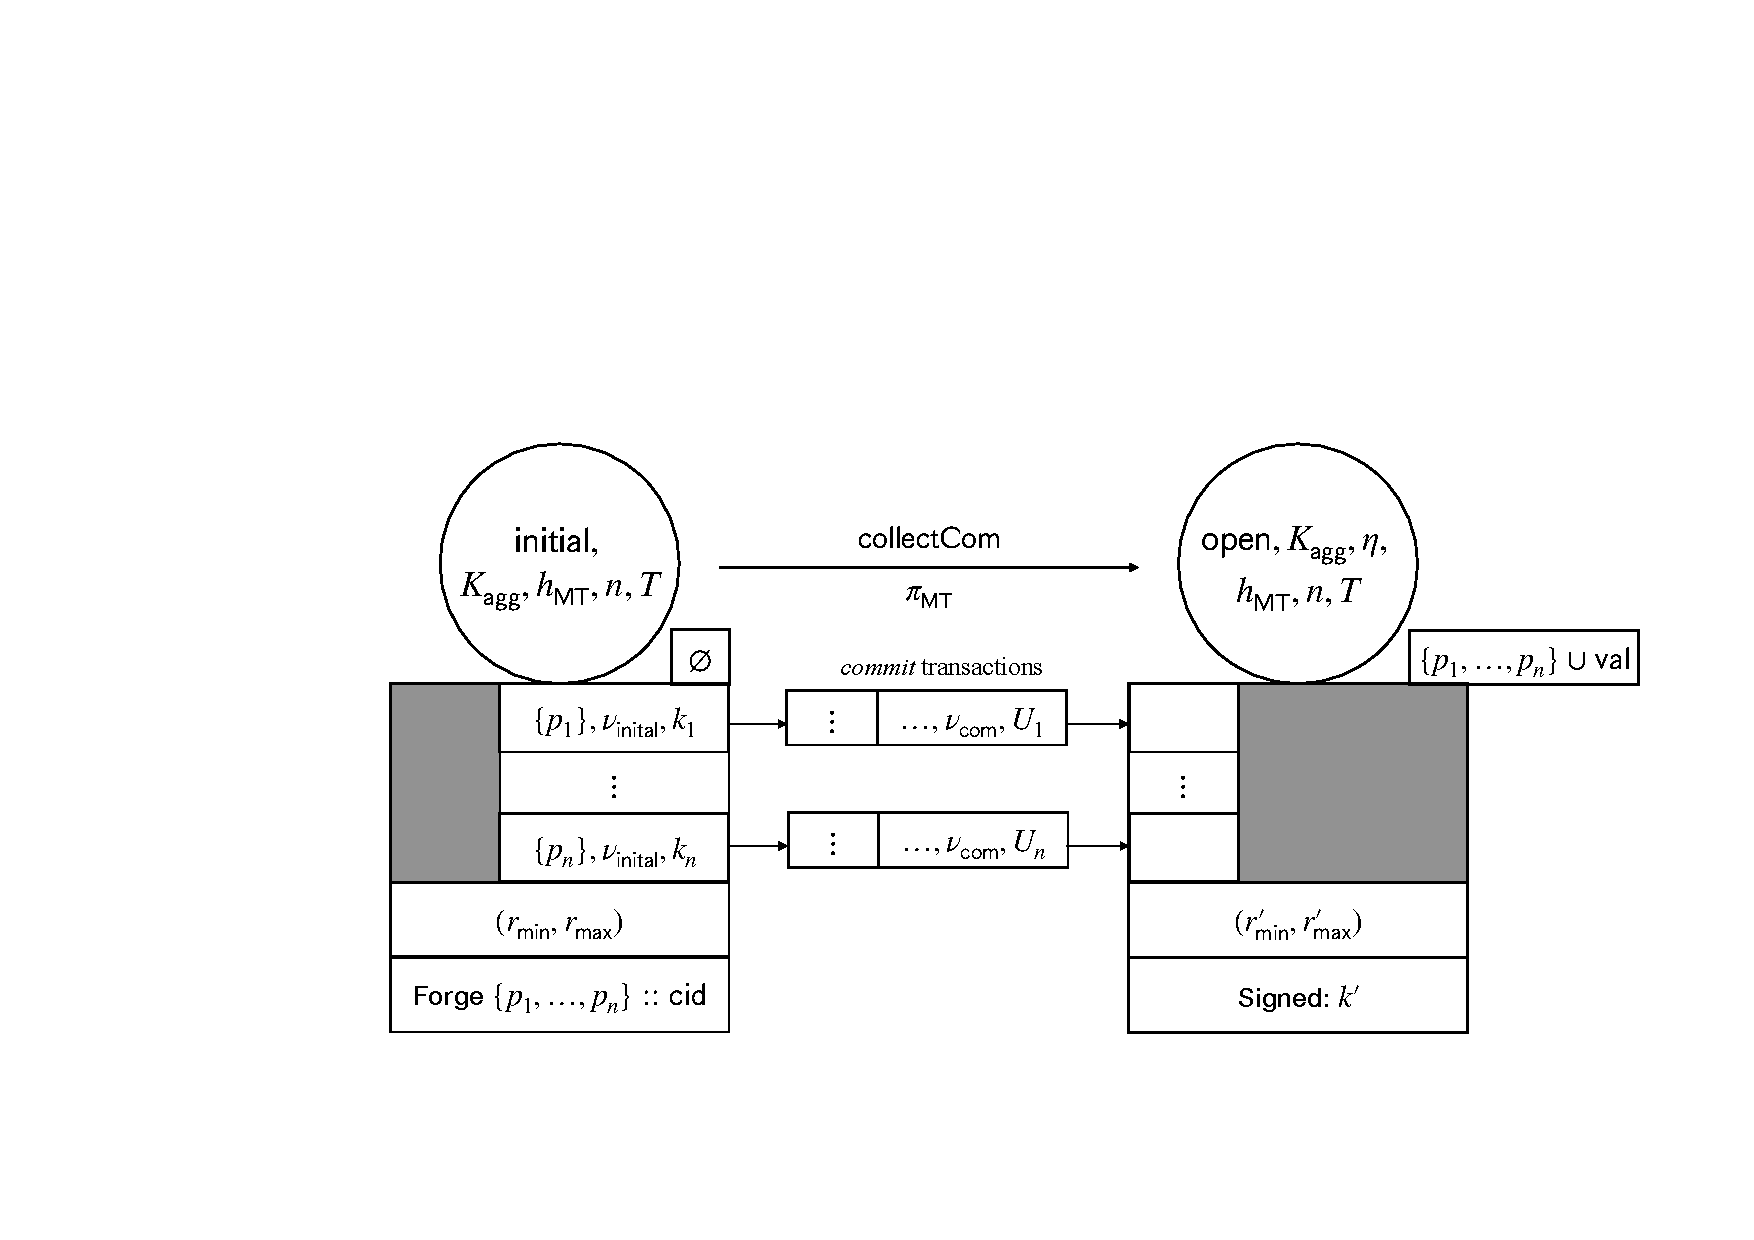
\includegraphics[width=\textwidth/2]{figures/SM_initial_open.pdf}
  %
  % TODO: clean draw marked up version
  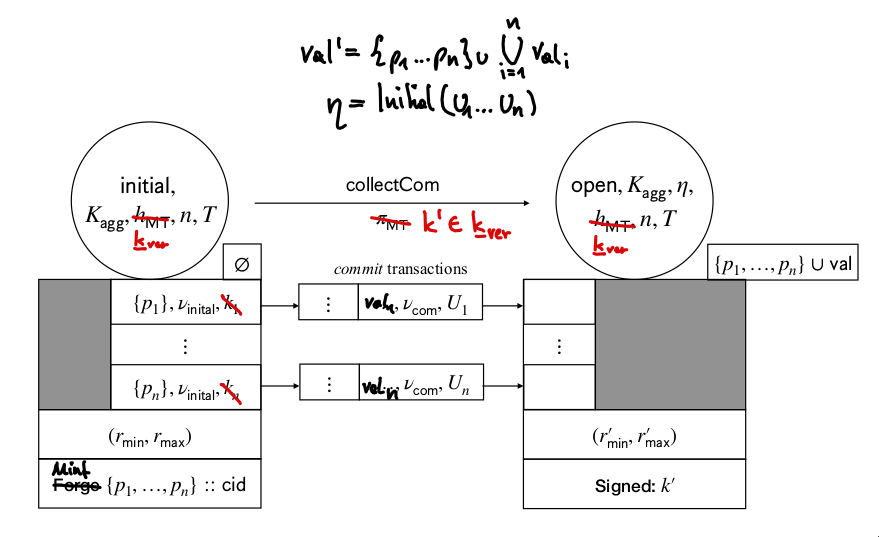
\includegraphics[width=\textwidth/2]{figures/SM_initial_open.png}

  \caption{\mtxInit{} transaction (left) with \mtxCCom{} transaction
    (right) and \mtxCom{} transactions (center).}
  \label{fig:SM_initial_open}

\end{figure}



%%% Local Variables:
%%% mode: latex
%%% TeX-master: "main"
%%% End:


\dparagraph{Collecting commits.} The SM transition from $\stInitial$ to
$\stOpen$ is achieved by posting the \mtxCCom{} transaction (see
Fig.~\ref{fig:SM_initial_open}). It needs to collect all previously committed
outputs (as well as the Head state input implied by the CEM model) and checks:

\begin{menumerate}
  \item committed UTxOs (datums) are recorded correctly in
  $\eta = \mathsf{Combine}(U_{1}, \ldots, U_{n})$,
  \item all committed value captured and no additional funds ``enter'' or ``leave''
  $\val' = \bigcup_{i=1}^{n} p_{i} \cup \val_{i}$,
  \item all tokens present in output
  $|\{cid \rightarrow . \rightarrow 1\} ~ \mathsf{in} ~ \val'| = \nop + 1$
  \todo{really count?},
  \item the transaction is signed by a verification key $k' \in \hppuv$ with its
  hash corresponding to the asset name of one of the participation tokens
  $\{p_1 \dots p_n\}$,
  \item unchanged parameters $\mathsf{cid}$, $\hpAK$, $\hppuv$, $\nop$, and
  $\cPer$ in the data field,
  \item no minting or burning happens.
\end{menumerate}

All parameters $\hpAK$, $\hppuv$, $\nop$, and $\cPer$ remain part of the state,
but in addition, a value $\eta \gets \ocvInitial(U_1,\ldots,U_n)$ is stored in
the state. The idea is that $\eta$ stores information about the initial UTxO
set, which is made up of the individual UTxO sets $U_i$ collected from the
commit transactions, in order to verify head-status information later (see
below).

It is also required that all $\nop$ participation tokens be present in the SM
output of the \mtxCollect{} transaction. This ensures that the \mtxCollect{}
transaction collects all $\nop$ commit transactions, because $\nuInitial$ does
not allow a \mtxCollect{} transaction to consume the outputs of the \mtxInit{}
transaction directly. The only way to post the \mtxCollect{} transaction is if
each head member has posted a \mtxCommit{} transaction.


\todo{WIP after here}

\dparagraph{Aborting a head.} The \mtxAbort{} transaction
(see Fig.~\ref{fig:SM_initial_final}) allows a party to abort the
creation of a head in case some parties fail to post a commit
transaction.  The final state does not contain any information (beyond
its identifier), but it is ensured that (1) the outputs $U$ correspond
to the union of all committed UTxO sets $U_i$ and (2) all
participation tokens are burned.


\begin{figure}

  \centering

  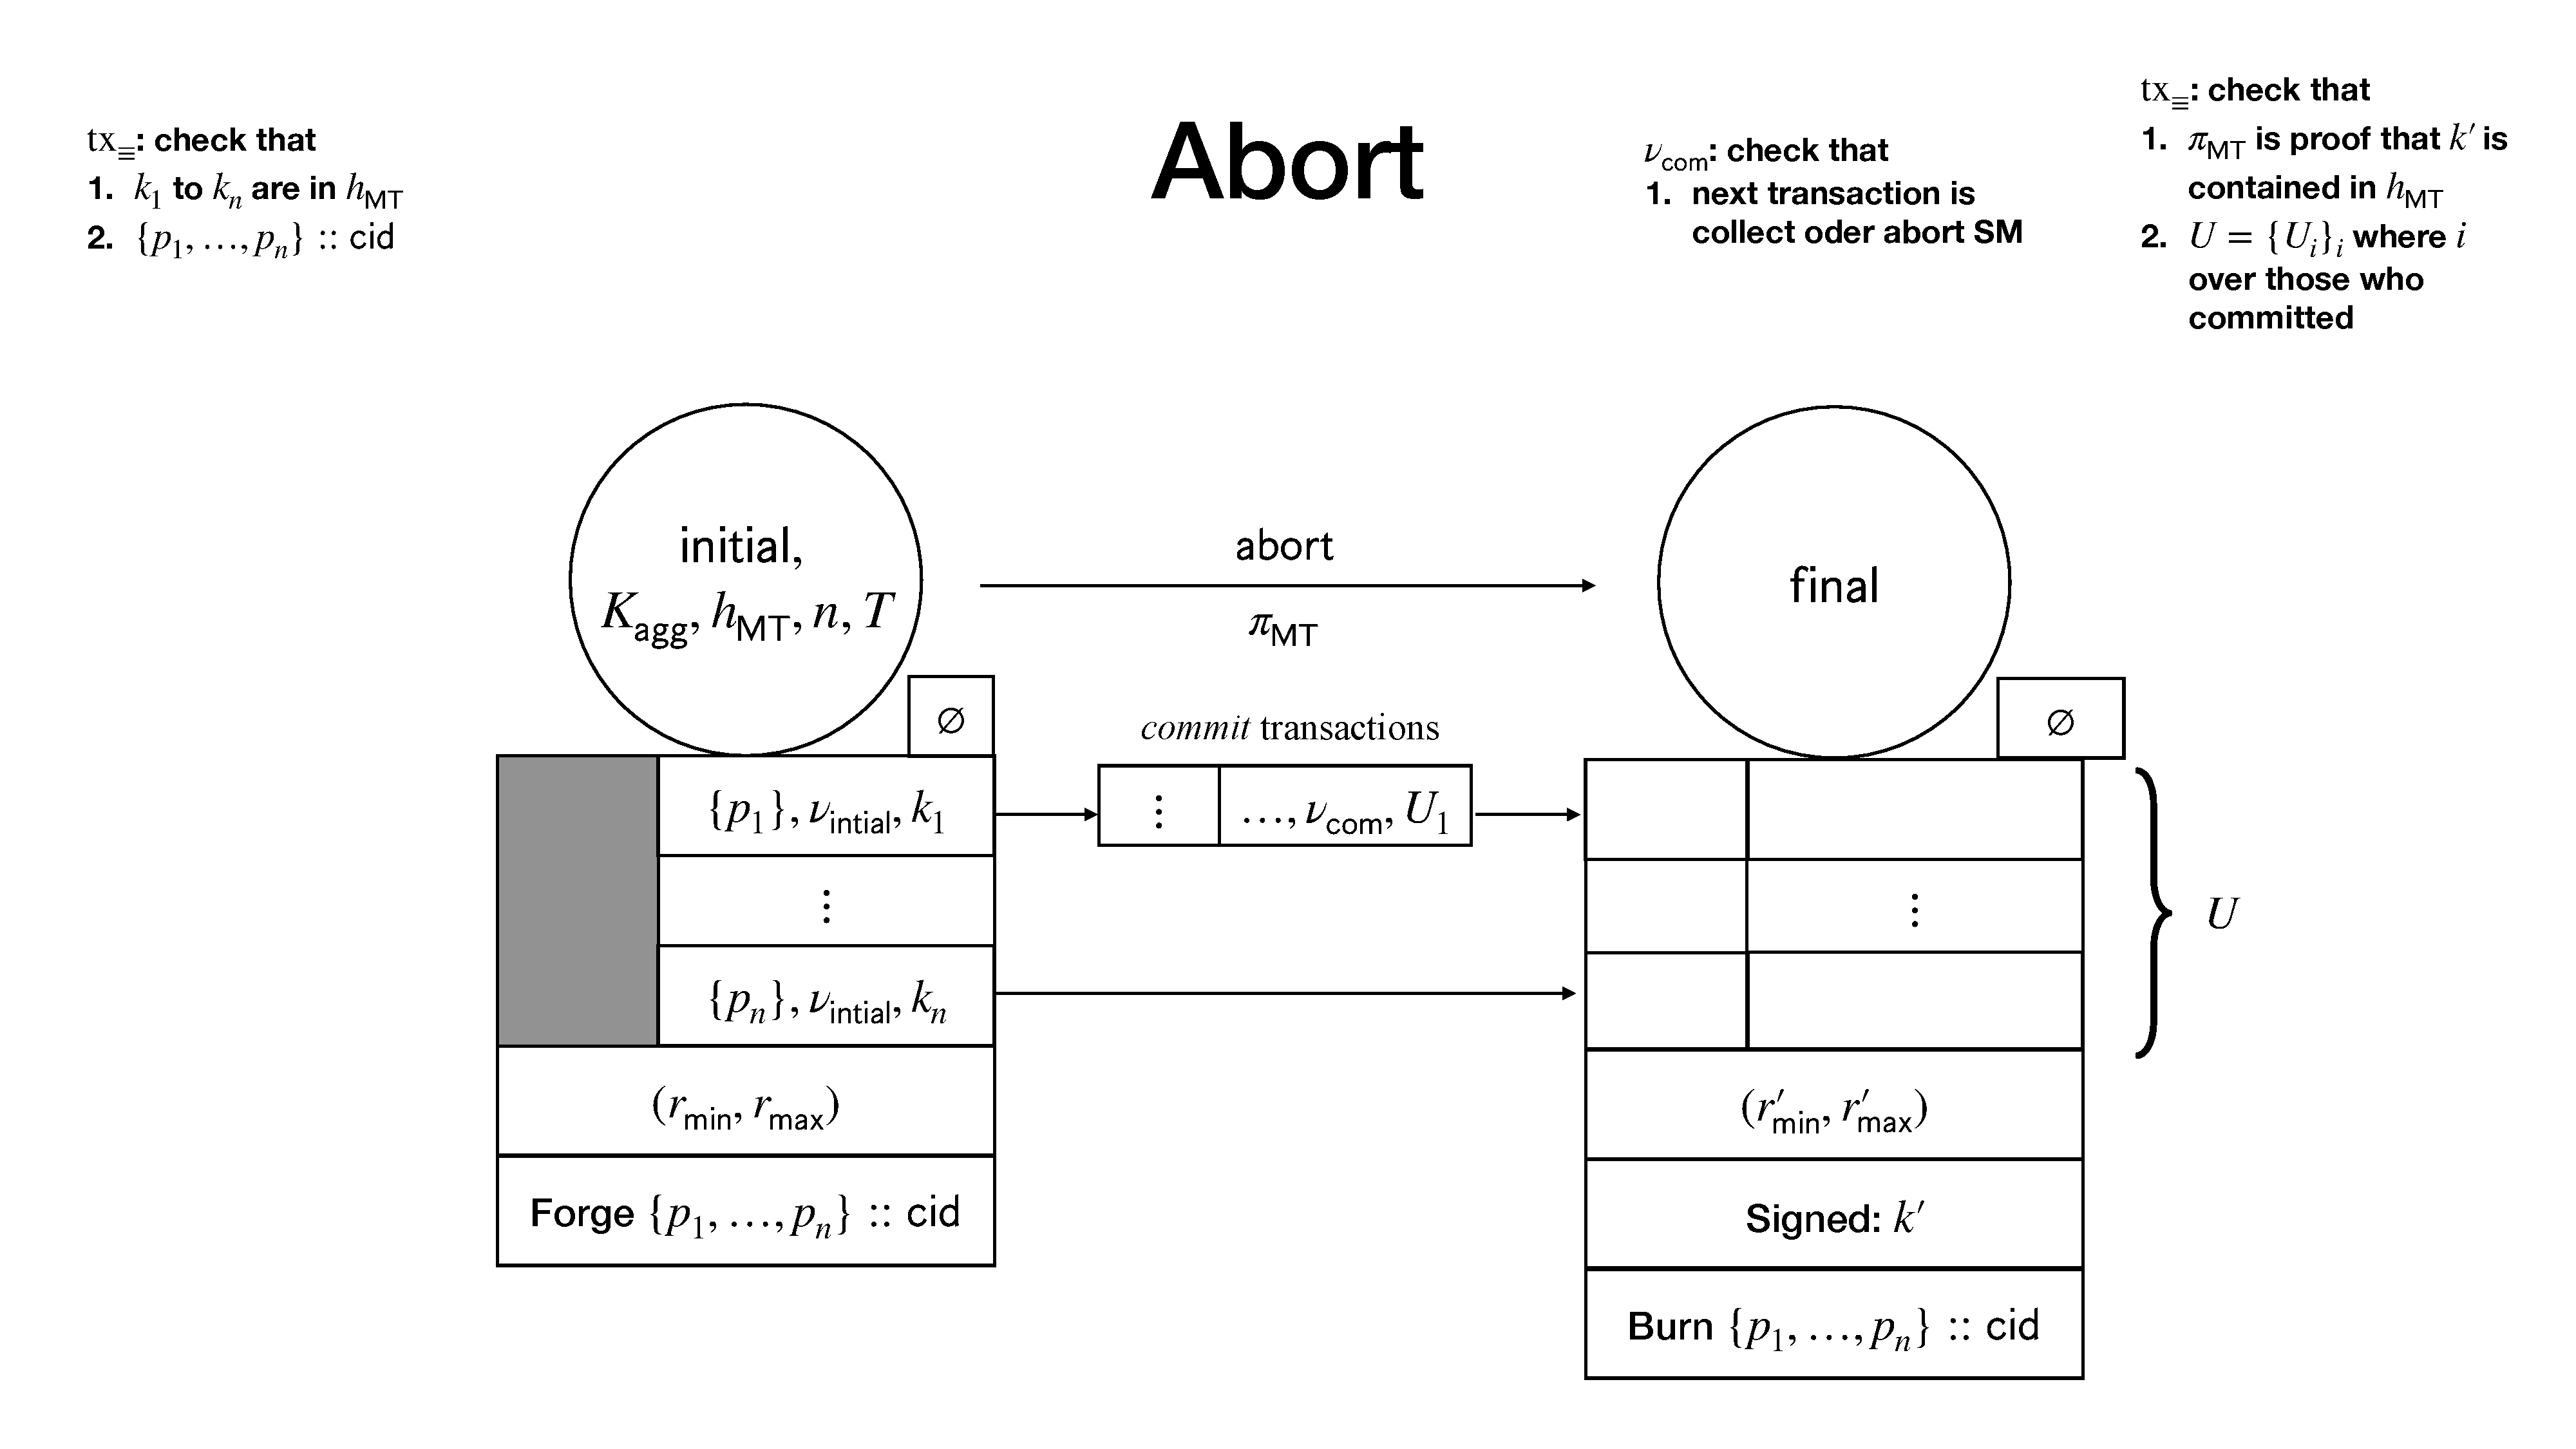
\includegraphics[width=\textwidth/2-2em,trim=350 20 240 300,
  clip]{figures/SM_initial_final.pdf}
    
  \caption{\mtxInit{} transaction (left) with \mtxAbort{} transaction
    (right) and \mtxCom{} transactions (center).}
  \label{fig:SM_initial_final}

\end{figure}



%%% Local Variables:
%%% mode: latex
%%% TeX-master: "main"
%%% End:



\dparagraph{Close transaction.} In order to close a head, a head
member may post the \mtxClose{} transaction (see
Fig.~\ref{fig:SM_open_closed}), which results in a state transition
from the $\stOpen$ state to the $\stClosed$ state.  For a successful
close, a head member must provide valid information $\xi$ about (their
view of) the current head state.  This information is passed through
OCV algorithm $\ocvClose$, resulting in a new OCV status
$\eta' \gets \ocvClose(\hpAK,\eta,\xi)$.  OCV algorithm $\ocvClose$
uses the previous OCV status $\eta$ and $\hpAK$ to check the head
information~$\xi$.  Note that if a check fails, $\ocvClose$ may output
$\bot$, but in order for a \mtxClose{} transaction to be valid,
$\eta' \neq \bot$ is required.

Once a \mtxClose{} transaction has been posted, a \emph{contestation period}
begins which should last at least $\cPer$ slots.  Hence, the last slot
$\Tfinal$ of the contestation period is recorded in the state, and it
is ensured that $\Tfinal \geq \txRmax' + \cPer$.

Finally, the SM state is extended by a set $\contesters$
initialized to the poster's signing key, i.e.,
$\contesters \gets \{k'\}$.   $\contesters$ is used to ensure that no party
posts more than once during the contestation period.


\begin{figure}[t!]

  \centering

  %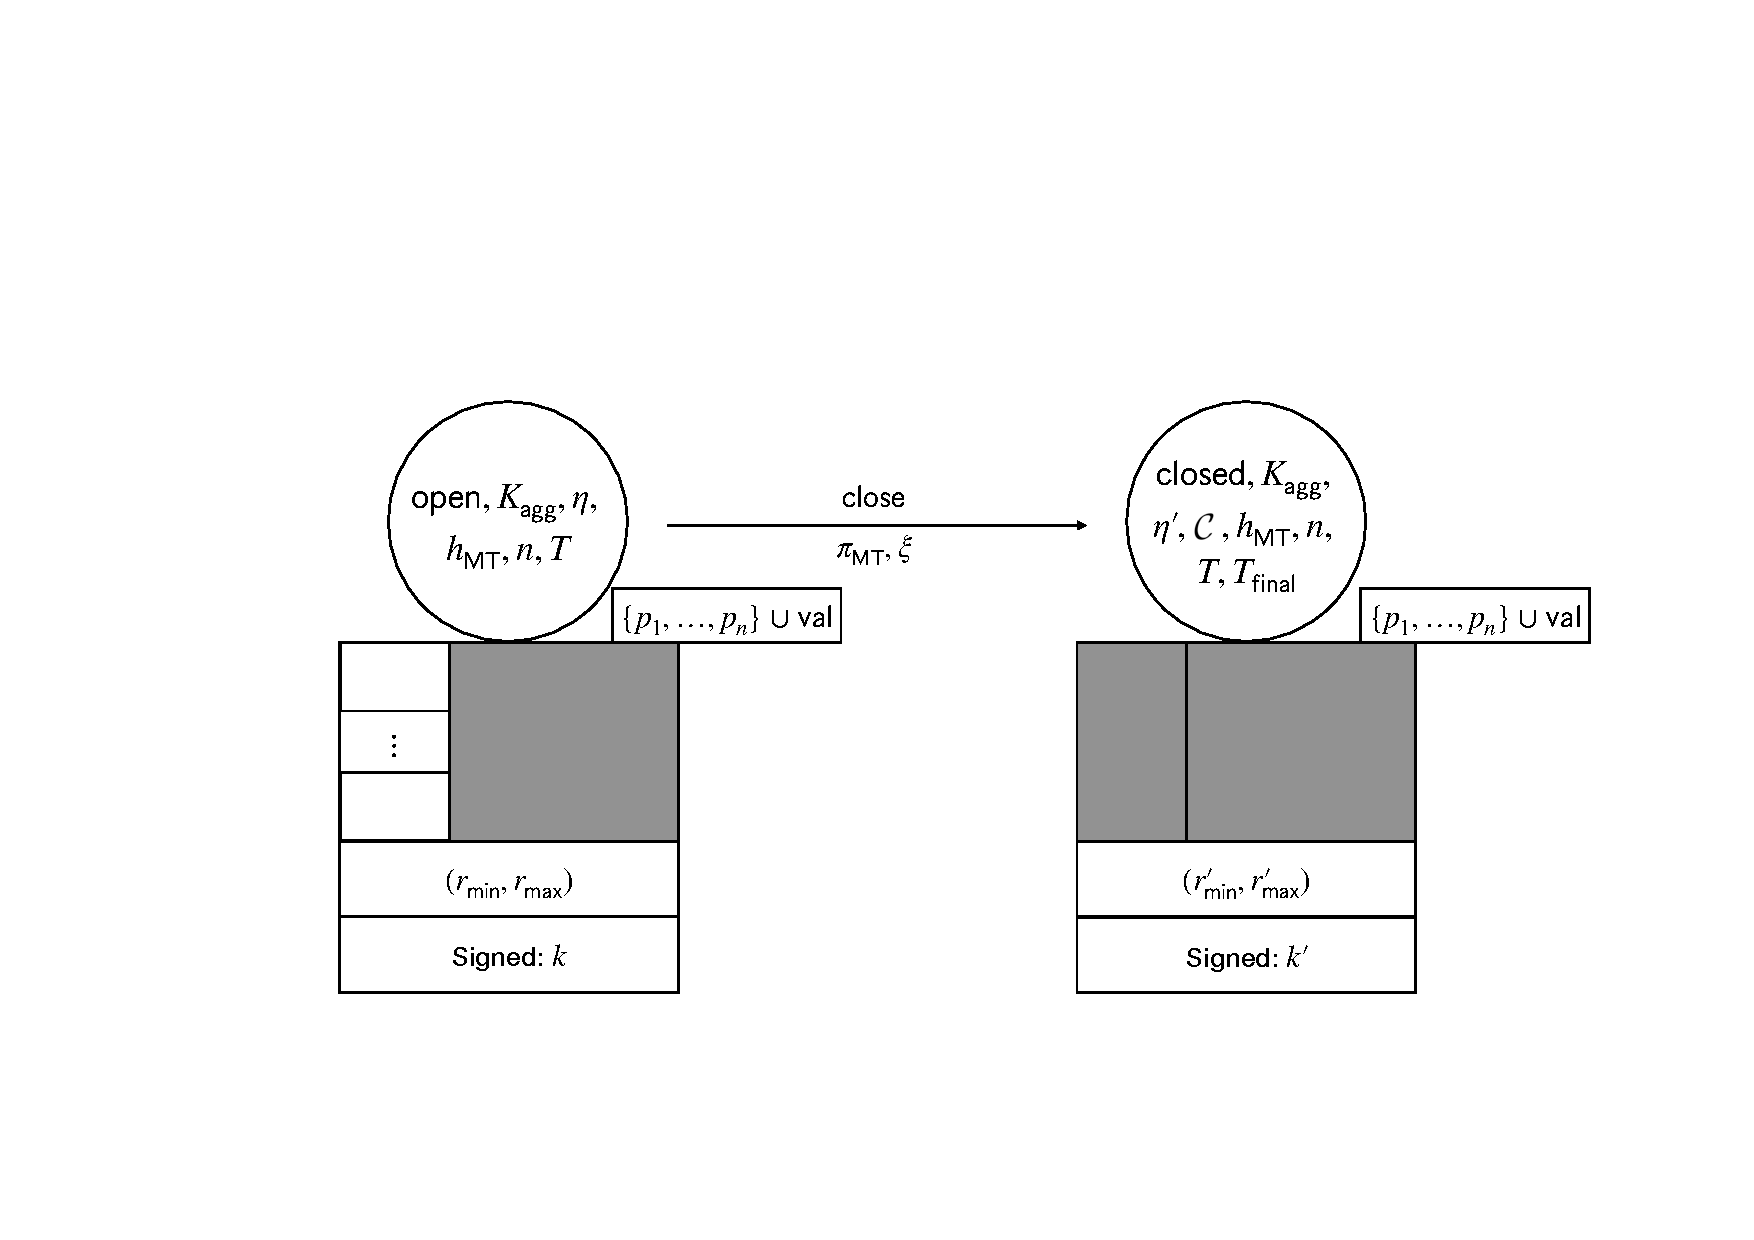
\includegraphics[width=\textwidth/2-2em,trim=350 100 160 300,
  %clip]{figures/SM_open_closed.pdf}

  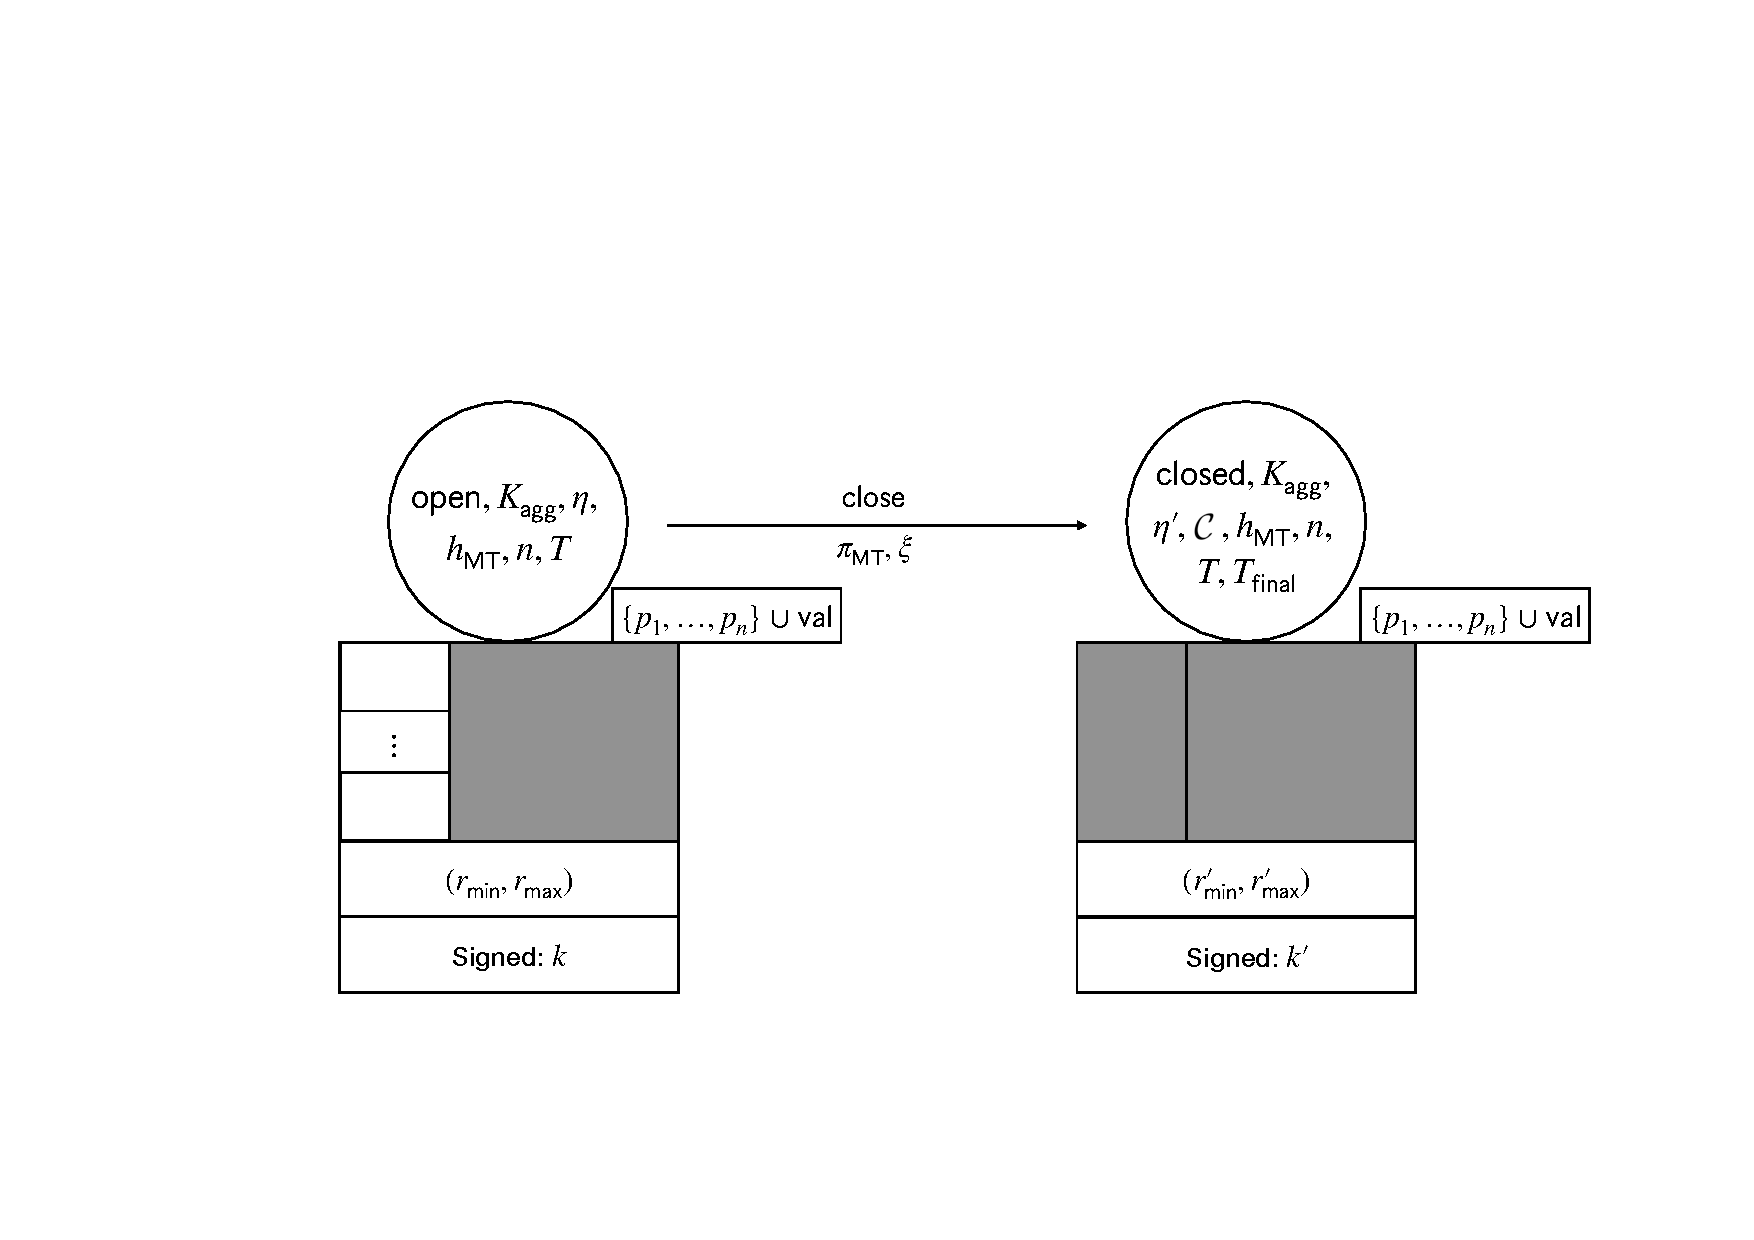
\includegraphics[width=\textwidth/2]{figures/SM_open_closed.pdf}

  \caption{\mtxCCom{} transaction (left) with \mtxClose{}
    transaction (right).}
  \label{fig:SM_open_closed}

\end{figure}



%%% Local Variables:
%%% mode: latex
%%% TeX-master: "main"
%%% End:



\dparagraph{Contestation.} If the party first closing a head posts
outdated/incomplete information about the current state of the head,
any other party may post a \mtxContest{} transaction (see
Fig.~\ref{fig:SM_closed_closed}), which causes a state transition from
the $\stClosed$ state to itself.  The transition handles update
information $\xi$ by passing it through OCV algorithm $\ocvContest$,
resulting in a new OCV status
$\eta' \gets \ocvContest (\hpAK,\eta,\xi)$.  OCV algorithm
$\ocvContest$ uses the previous OCV status $\eta$ and $\hpAK$ to check
the update information $\xi$.  Similarly to $\ocvClose$, $\ocvContest$
may output $\bot$, but in order for a \mtxContest{} transaction to be
valid $\eta' \neq \bot$ is required.

The \mtxContest{} transaction is only valid if the old set
$\contesters$ of parties who have contested (or closed) so far does not yet
include the poster, i.e., $k' \notin \contesters$.  If this check
passes, the set is extended to include the poster of the \mtxContest{}
transaction, i.e., $\contesters' \gets \contesters \cup \{k'\}$.
Furthermore, \mtxContest{} transactions may only be posted up until
$\Tfinal$, i.e., it is required that $\txRmax' \leq \Tfinal$.

Observe that during the contestation period, up to $\nop-1$
\mtxContest{} transactions may be posted (of course, the parameter
$\cPer$ has to be chosen large enough as to allow each head member to
potentially post a \mtxClose{}/\mtxContest{} transaction).


\begin{figure}

  \centering

  %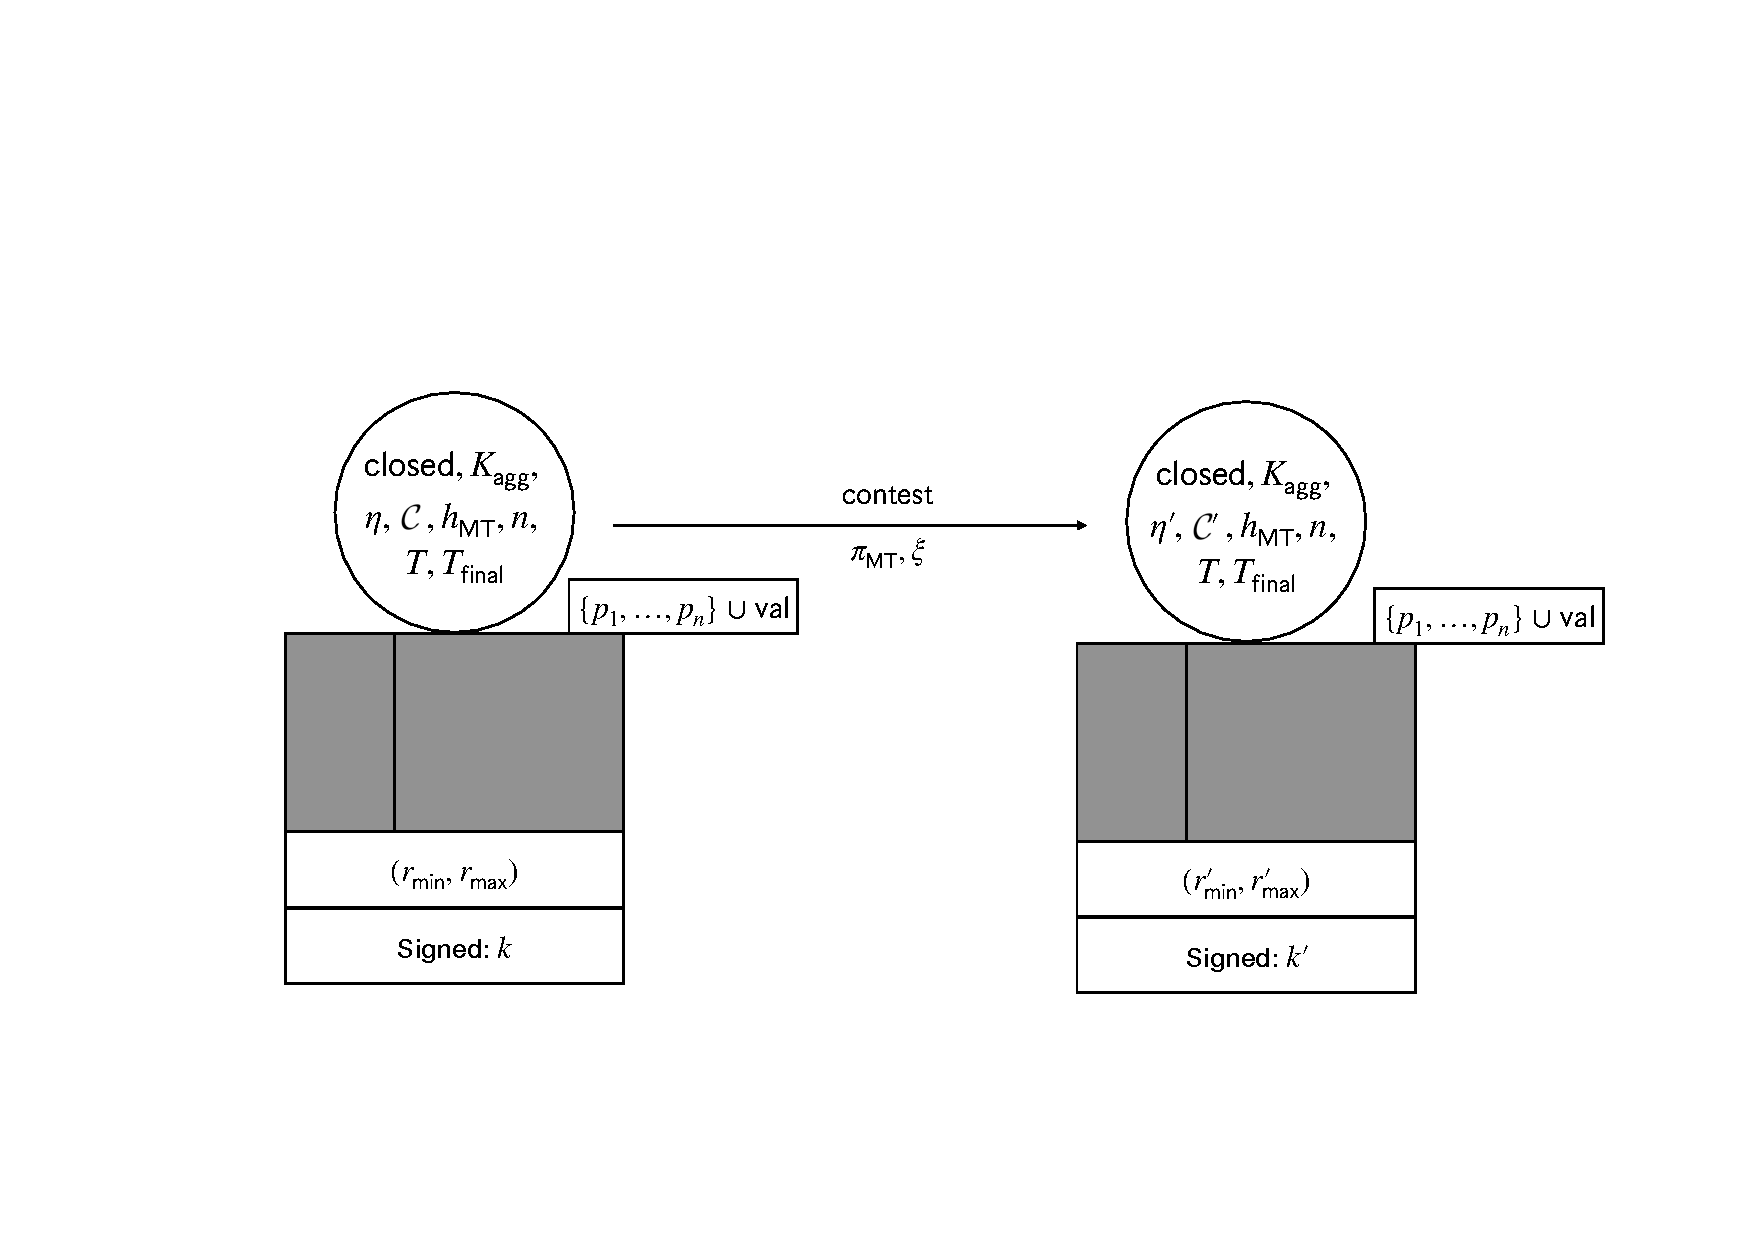
\includegraphics[width=\textwidth/2-2em,trim=280 120 160 260,
  %clip]{figures/SM_closed_closed.pdf}

  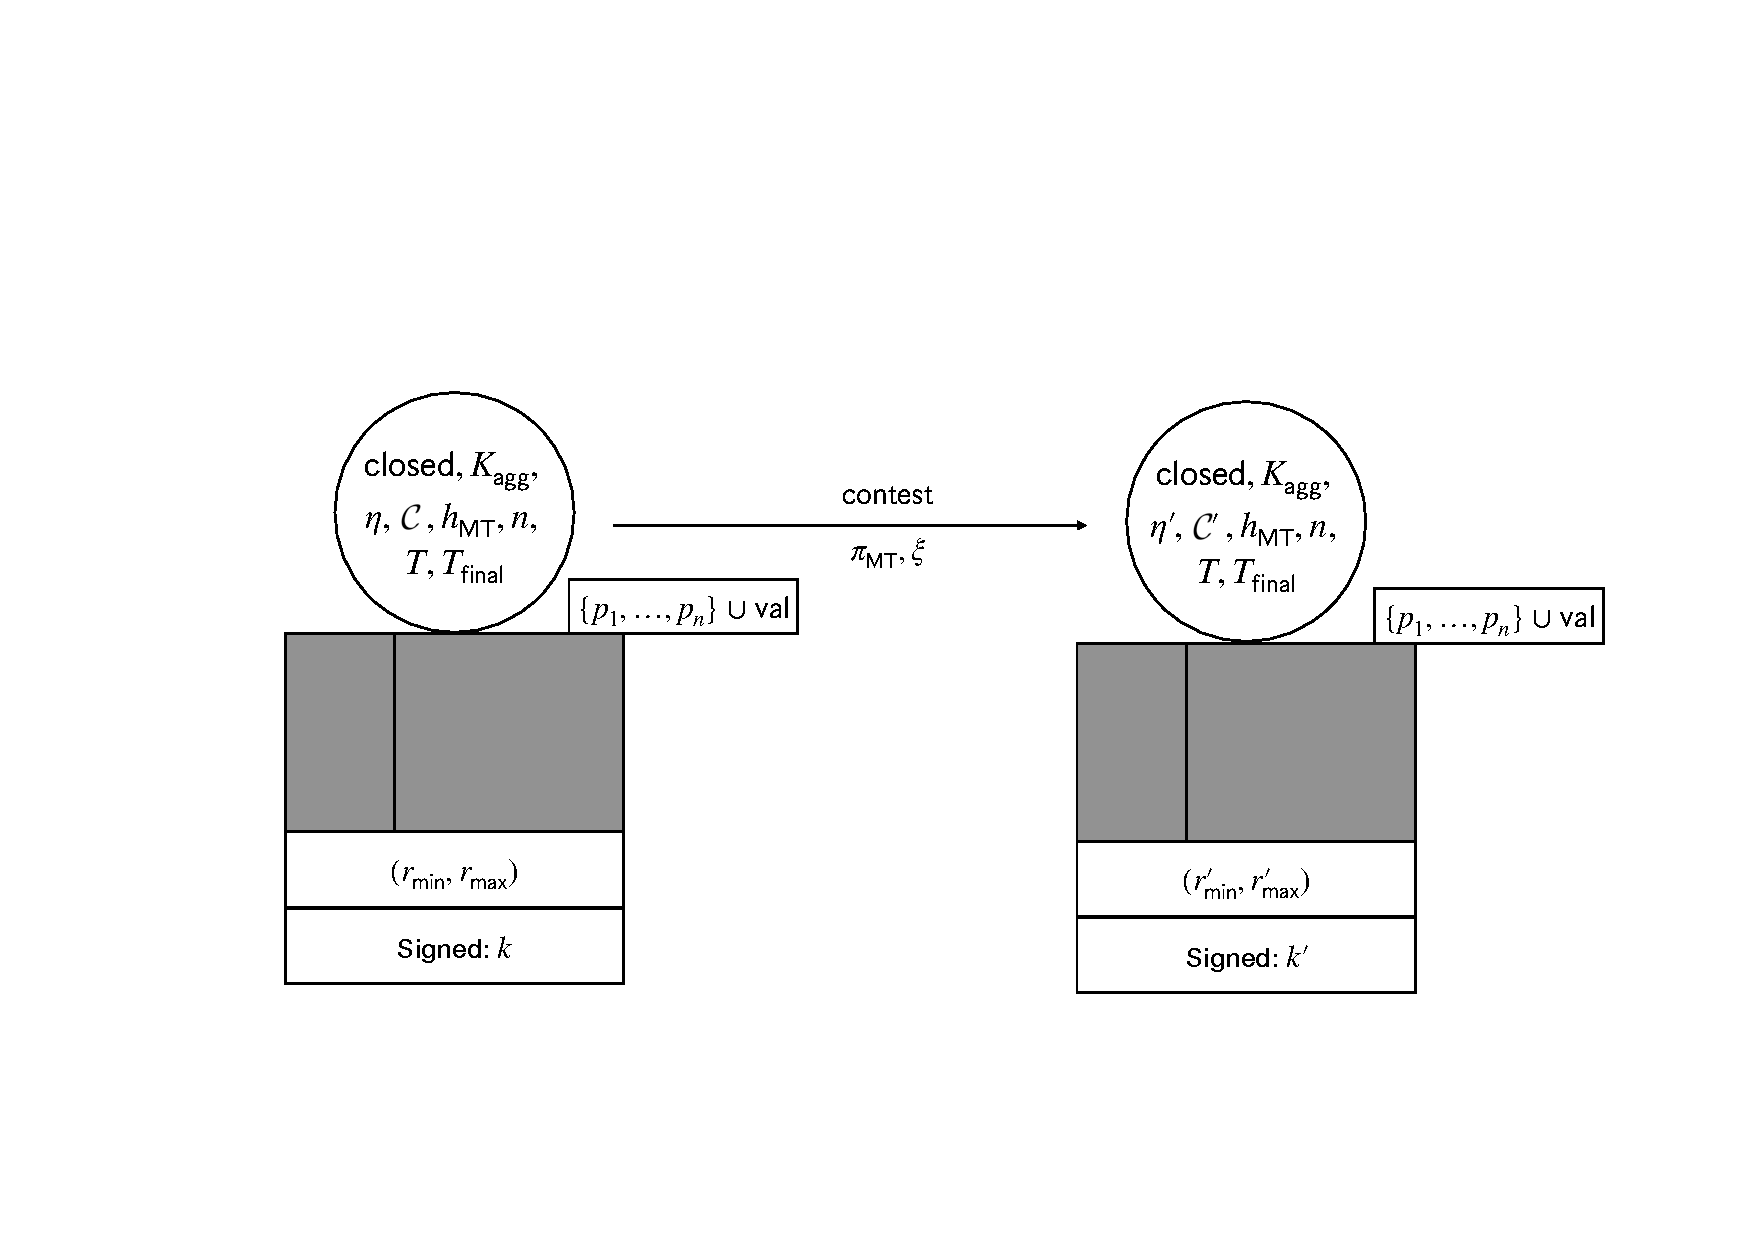
\includegraphics[width=\textwidth/2]{figures/SM_closed_closed.pdf}

  \caption{\mtxClose{}/\mtxContest{} transaction (left);
    \mtxContest{} transaction (right)}
  \label{fig:SM_closed_closed}

\end{figure}



%%% Local Variables:
%%% mode: latex
%%% TeX-master: "main"
%%% End:


\begin{figure}

  \centering

  % 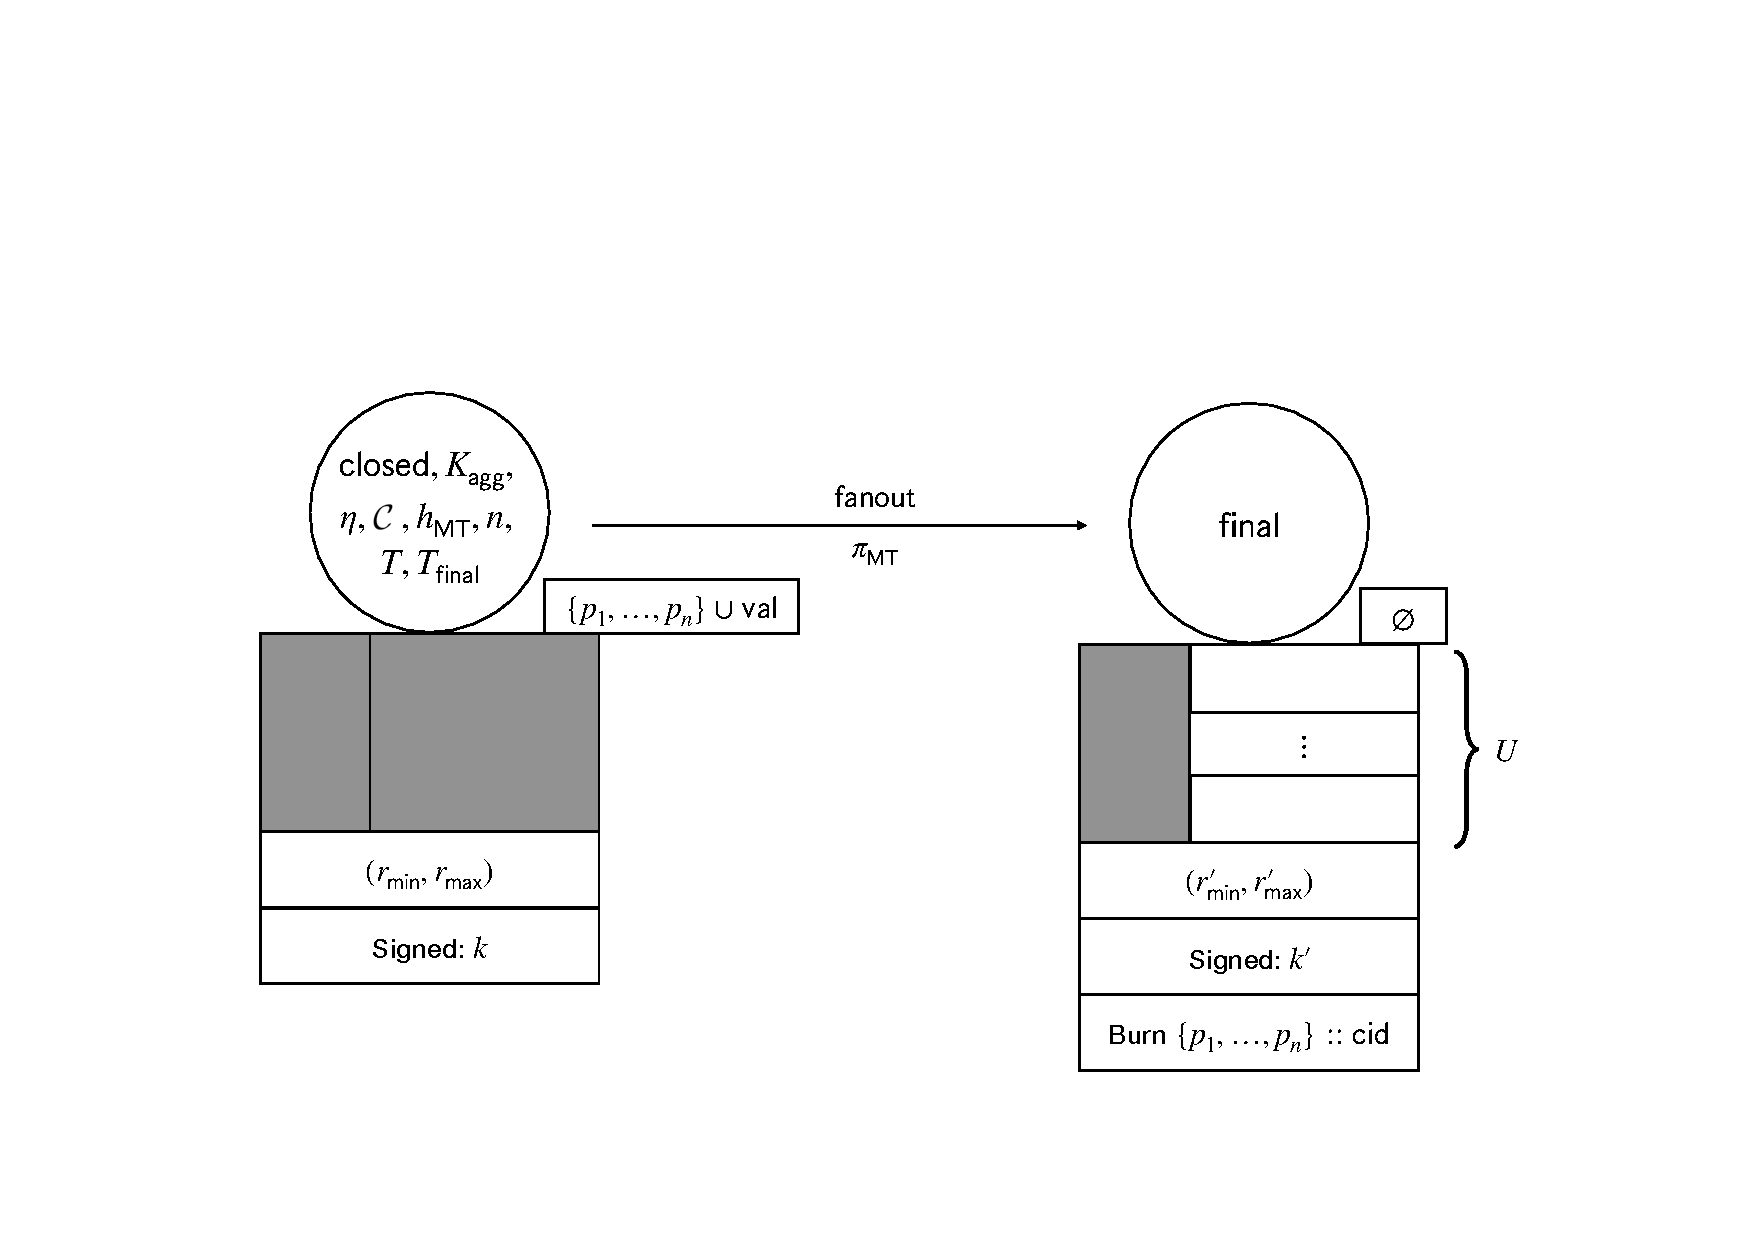
\includegraphics[width=\textwidth/2]{figures/SM_closed_final.pdf}

  % TODO: clean draw marked up version
  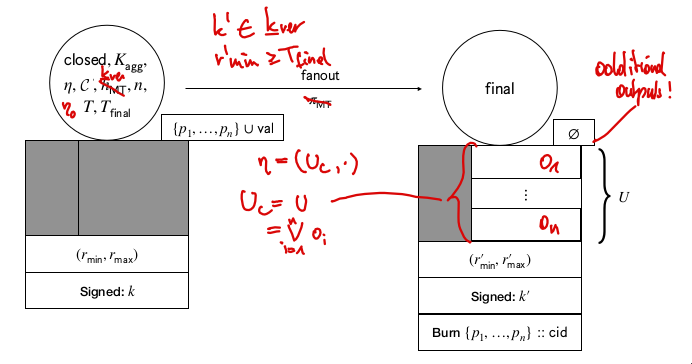
\includegraphics[width=\textwidth/2]{figures/SM_closed_final.png}

  \caption{\mtxClose{}/\mtxContest{} transaction (left);
    \mtxFanout{} transaction (right)}\label{fig:SM_closed_final}

\end{figure}

%%% Local Variables:
%%% mode: latex
%%% TeX-master: "main"
%%% End:


\dparagraph{Final state.}  Once the contestation phase is over, a head
may be finalized by posting a \mtxFanout{} transaction, taking the SM
from $\stClosed$ to $\stFinal$.  The \mtxFanout{} transaction must
have outputs that correspond to the most recent head state.  To that
end, OCV predicate $\ocvFinal$ checks the transaction's output set $U$
against the information recorded in $\eta$.  The \mtxFanout{}
transaction is only valid if $\ocvFinal$ outputs $\true$.  Moreover,
to ensure that the \mtxFanout{} transaction is not posted too early,
$\txRmin' > \Tfinal$ is required.  Finally, all participation tokens
must be burned.


%%% Local Variables:
%%% mode: latex
%%% TeX-master: "main"
%%% End:
